\documentclass[12pt]{article}
\pagestyle{empty}
\usepackage[margin=0.75in]{geometry}
\usepackage{fullpage}
\usepackage{graphicx}
\usepackage{subcaption}
\usepackage{amsmath}
\usepackage{amsfonts}
\usepackage{listings}
\usepackage{color}
\usepackage{textcomp}
\definecolor{listinggray}{gray}{0.9}
\definecolor{lbcolor}{rgb}{0.9,0.9,0.9}
\lstset{
	backgroundcolor=\color{lbcolor},
	tabsize=4,
	rulecolor=,
% 	language=Python,
        basicstyle=\scriptsize,
        upquote=true,
        aboveskip={1.5\baselineskip},
        columns=fixed,
        showstringspaces=false,
        extendedchars=true,
        breaklines=true,
        prebreak = \raisebox{0ex}[0ex][0ex]{\ensuremath{\hookleftarrow}},
        frame=single,
        showtabs=false,
        showspaces=false,
        showstringspaces=false,
        identifierstyle=\ttfamily,
        keywordstyle=\color[rgb]{0,0,1},
        commentstyle=\color[rgb]{0.133,0.545,0.133},
        stringstyle=\color[rgb]{0.627,0.126,0.941},
}

% \title{Stabilized FEM Homework 3}
% \author{Truman Ellis}
% \date{}

\begin{document}
\section*{Problem 2.8}
\begin{figure}[h!]
\centering
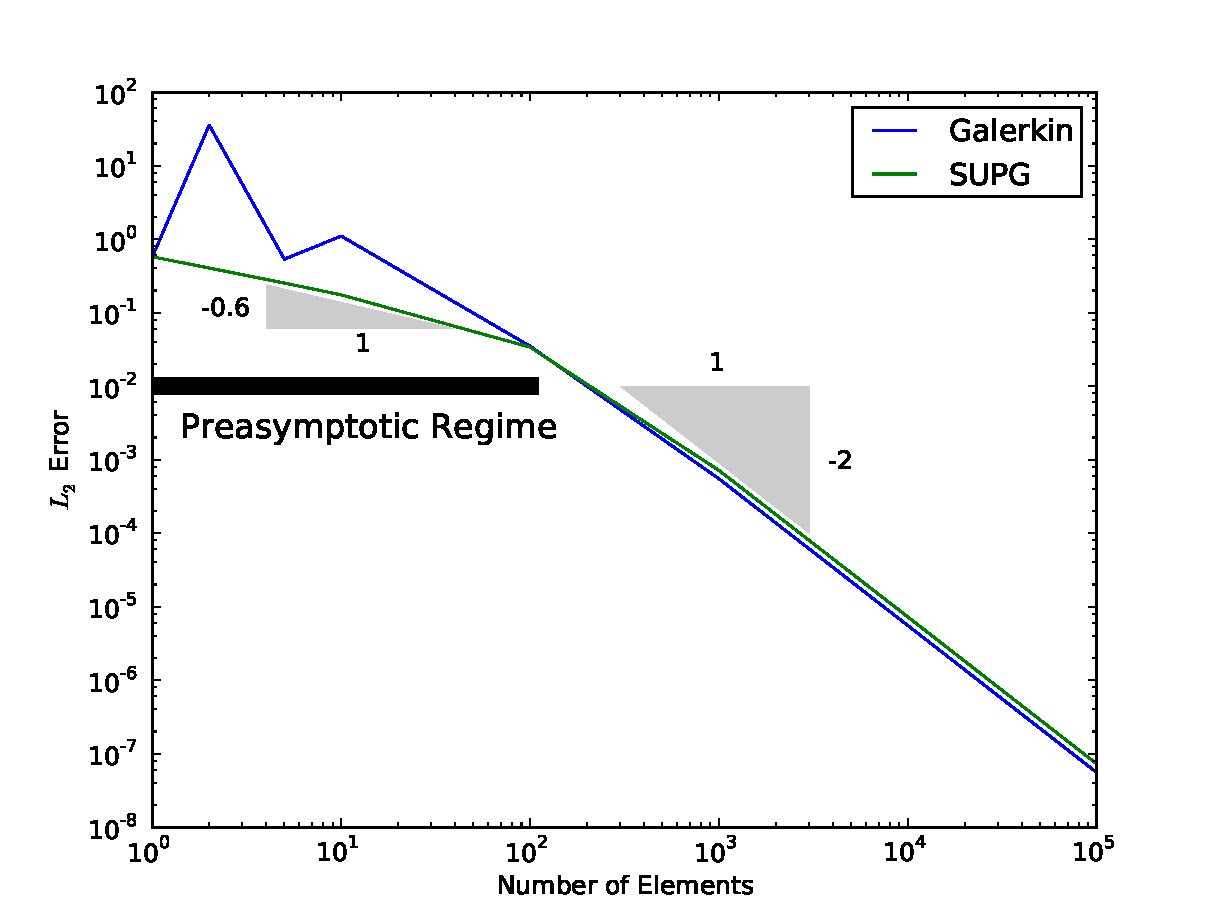
\includegraphics[width=0.8\textwidth]{L2Norm.pdf}
\end{figure}

\begin{figure}[h!]
\centering
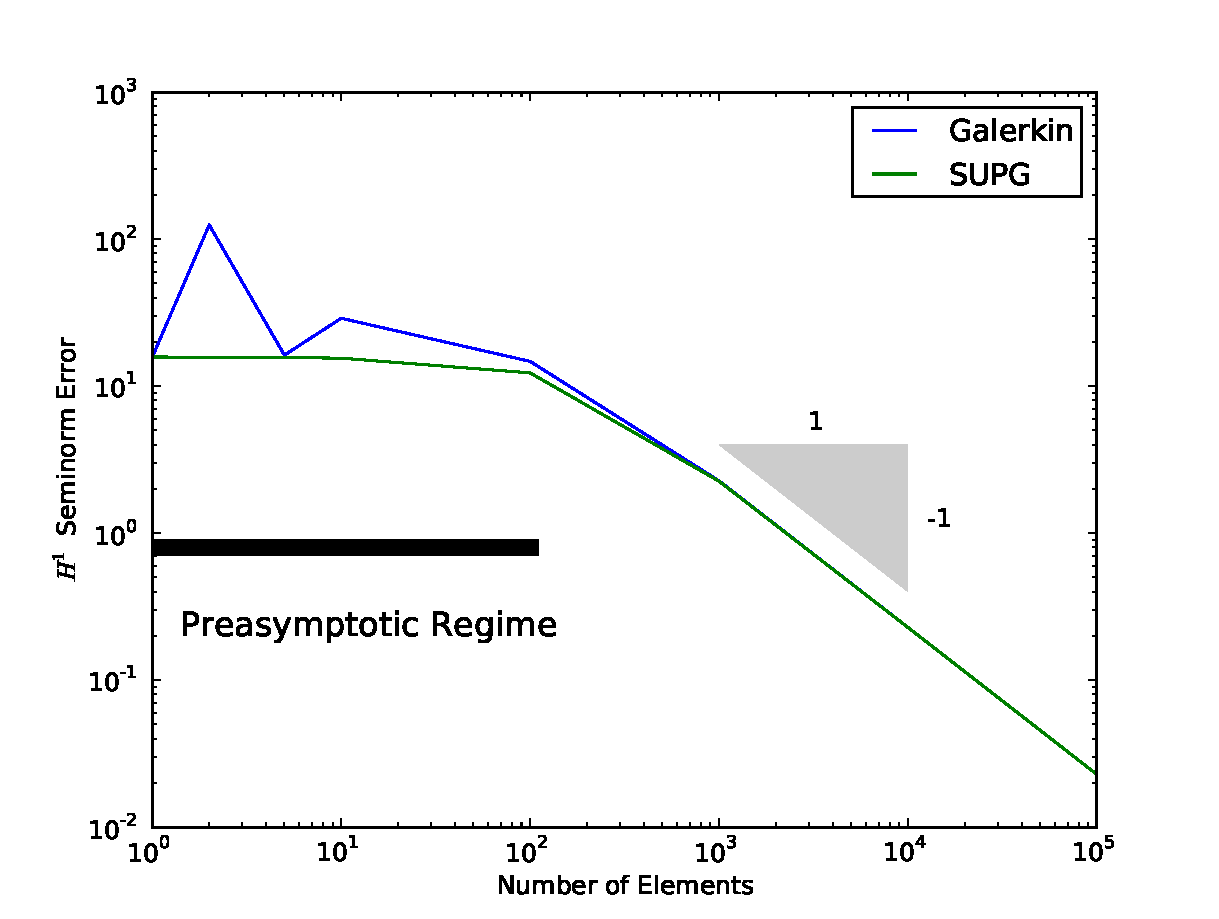
\includegraphics[width=0.8\textwidth]{H1Seminorm.pdf}
\end{figure}

\begin{figure}[h!]
\centering
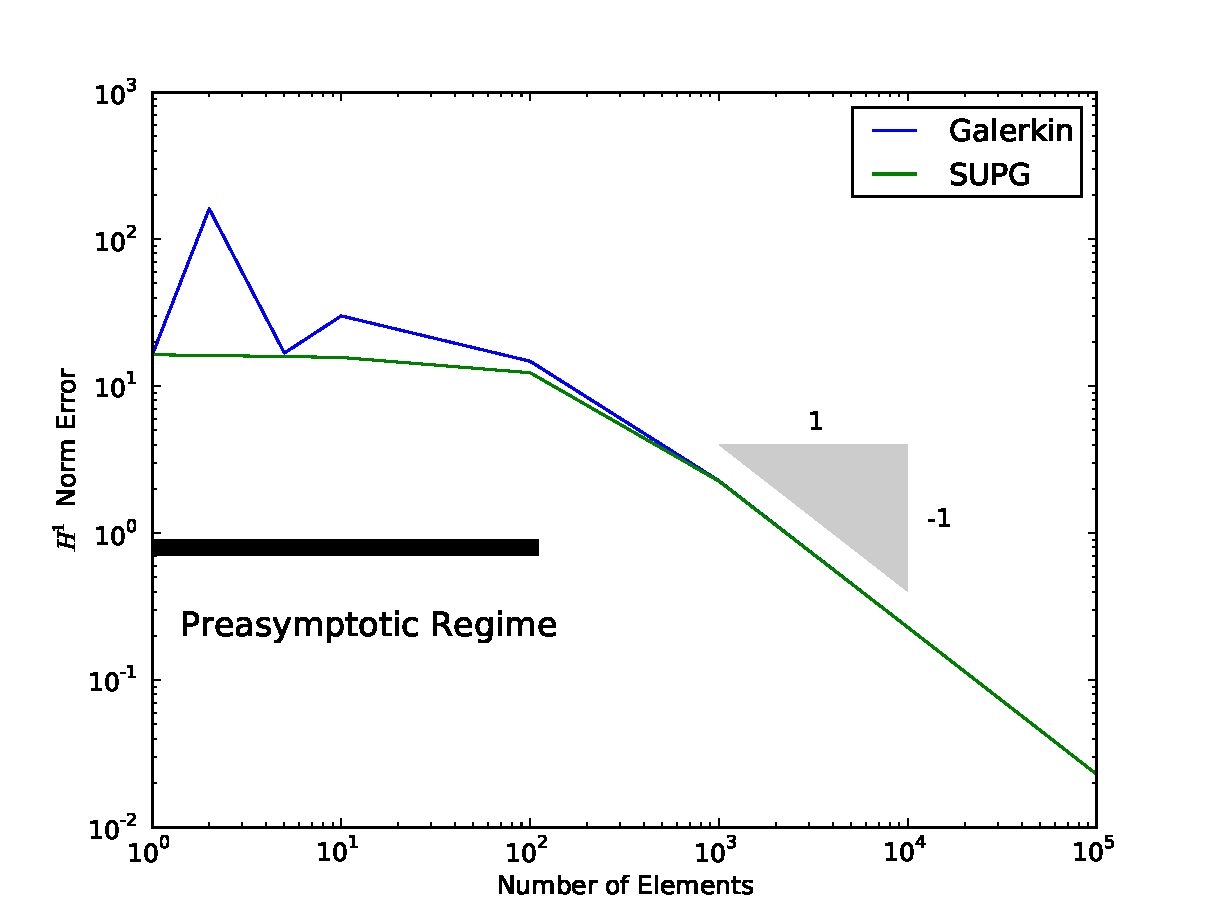
\includegraphics[width=0.8\textwidth]{H1Norm.pdf}
\end{figure}

The biggest difference between the Galerkin and SUPG convergence plots is that
SUPG has monotone error convergence in both the $L_2$ and $H^1$ sense, whereas
the Galerkin error, like the solution, oscillates badly in the preasymptotic
regime. Eventually, the Galerkin method begins to work as the element Peclet
number goes down, but it is pretty oscillatory until then. The two methods
eventually converge with the same rate, but the absolute value of error in the
preasymptotic regime is much better for SUPG. The $L_2$ error of the SUPG
solution starts slowly with a fractional slope of approximately 0.6 before it
accelerates to a  convergence rate of 2.0. The convergence rate for the
solution derivative on the other hand starts out nearly stagnant before
jumping to a rate of 1.0 outside of the preasymptotic regime. The Galerkin error is too
oscillatory in the coarse meshes to identify a well-defined convergence rate,
but it too reaches 2.0 on finer meshes. Similarly, the derivative error
oscillates preasymptotically before reaching a rate of 1.0. The $H^1$ error is
dominated by the $H^1$ seminorm error and we thus get nearly identical plots
for both SUPG and Galerkin.

\clearpage
\lstinputlisting[language=Python,title={Problem 2.8 Code}]{HW28.py}

\end{document}

